\section{Experiments}\label{sec:exp}

\subsection{Heuristics}
We designed many heuristics for both A* and RBFS. Here we show an admissible one and two non-admissible ones for demonstration. Other heuristics will be discussed in section \ref{sec:dis}.

We designed an admissible heuristic by reasonning about simulating the game of tower. For the second and third peg, disks on there should intuitively be moved to the first peg to get to the goal state. An admissible estimation of steps is the amount of disks in these pegs. If a disk at the bottom of the first peg is not the right one, it should be moved out first and then move to its ideal position, which takes at least $2k$ steps, where k is the number of disks on top of it. We show the heuristic below:
\[
h1(s) = I(s(1,0)==goal(1,0))\cdot 2 \cdot num(s(1)) + num(s(2)) + num(s(3))
\]
Here $I(\cdot)$ is indication function, and $num(\cdot)$ is the function for counting disks.

A non-trivial non-admissible heuristic is designed in a similar way but taking ordering into account:
\[
h2(s) = (\sum_i |s(1,i)-i| ) + numberDisks(s(2)) + numberDisks(s(3))
\]
Here s(i,j) is the $jth$ disk in peg $i$ (pegs indexed 0 to 2 from left to right here). The intuition is that for a disk $k$ in peg $1$, it has to take $|k-i|$ steps to get to the $kth$ place by moving away or filling out disks on peg $0$, where $i$ is its current location on the peg. For example, if the $9th$ disk is on the bottom, it has to take 9 minus 0 steps to get to the top. For disks on peg $2$ and peg $3$, they have to be moved from the current location to peg $1$ in at least $1$ step, which is the same as the admissible heuristic. However this is not an admissible heuristic because there are multiple counts for disks on peg $0$. 

For a fast non-admissible heuristic, we simplily enlarge the former heuristic by a factor of $2$. We will see that this relaxation makes the increasing of computation and expanded nodes become linear in the problem size ranging from $4-10$.
\[
h3(s) = 2 \cdot [(\sum_i |s(1,i)-i| ) + numberDisks(s(2)) + numberDisks(s(3))]
\]
\subsection{Results}

\begin{figure}[!t]
\centering
\begin{tabular}{cc}
\subfloat[A* nodes: all 140 experiments]{\includegraphics[scale=0.32]{img/tnode_Astar.pdf}} 
   & \subfloat[RBFS nodes: all 140 experiments]{\includegraphics[scale=0.32]{./img/tnode_RBFS.pdf}}\\
\subfloat[A* average searched nodes]{\includegraphics[scale=0.32]{./img/anode_Astar.pdf}} 
   & \subfloat[RBFS average searched nodes]{\includegraphics[scale=0.32]{./img/anode_RBFS.pdf}}\\
%\subfloat[E]{\includegraphics[width=2cm]{logo}} 
%   & \subfloat[F]{\includegraphics[width=3cm]{logo}}\\
\end{tabular}
\caption{Plots for the number of nodes searched against the problem size for each algorithm and heuristic. For the first 2 figures, for each number of disks 4 to 10, every 20 examples have the same problem size.  We show the average number of expanded nodes against the number of disks for a clear demonstration. As the problem size becomes larger, the number of searched nodes grows exponentially.}
\label{fig:nodes}
\end{figure}

\begin{figure}[!t]
\centering
\begin{tabular}{cc}
\subfloat[A*: average cpu time (s) on heuristics]{\includegraphics[scale=0.32]{./img/AHcpu-aver.pdf}} 
   & \subfloat[RBFS: average cpu time (s) on heuristics]{\includegraphics[scale=0.32]{./img/RHcpu-aver.pdf}}\\
\subfloat[A*: average cpu time (s) on whole problem]{\includegraphics[scale=0.32]{./img/ATcpu-aver.pdf}} 
   & \subfloat[RBFS: average cpu time (s) on whole problem]{\includegraphics[scale=0.32]{./img/RTcpu-aver.pdf}}\\
%\subfloat[E]{\includegraphics[width=2cm]{logo}} 
%   & \subfloat[F]{\includegraphics[width=3cm]{logo}}\\
\end{tabular}
\caption{Plots for the average cpu time against the problem size over 20 examples for each algorithm and heuristic.}
\label{fig:cputime}
\end{figure}

\begin{figure}[!t]
\centering
\begin{tabular}{cc}
\subfloat[Nodes against disks for admissible heurisitic]{\includegraphics[scale=0.32]{./img/node_Astar_RBFS_H_ad.pdf}} 
   & \subfloat[Nodes against disks for non-admissible heurisitic]{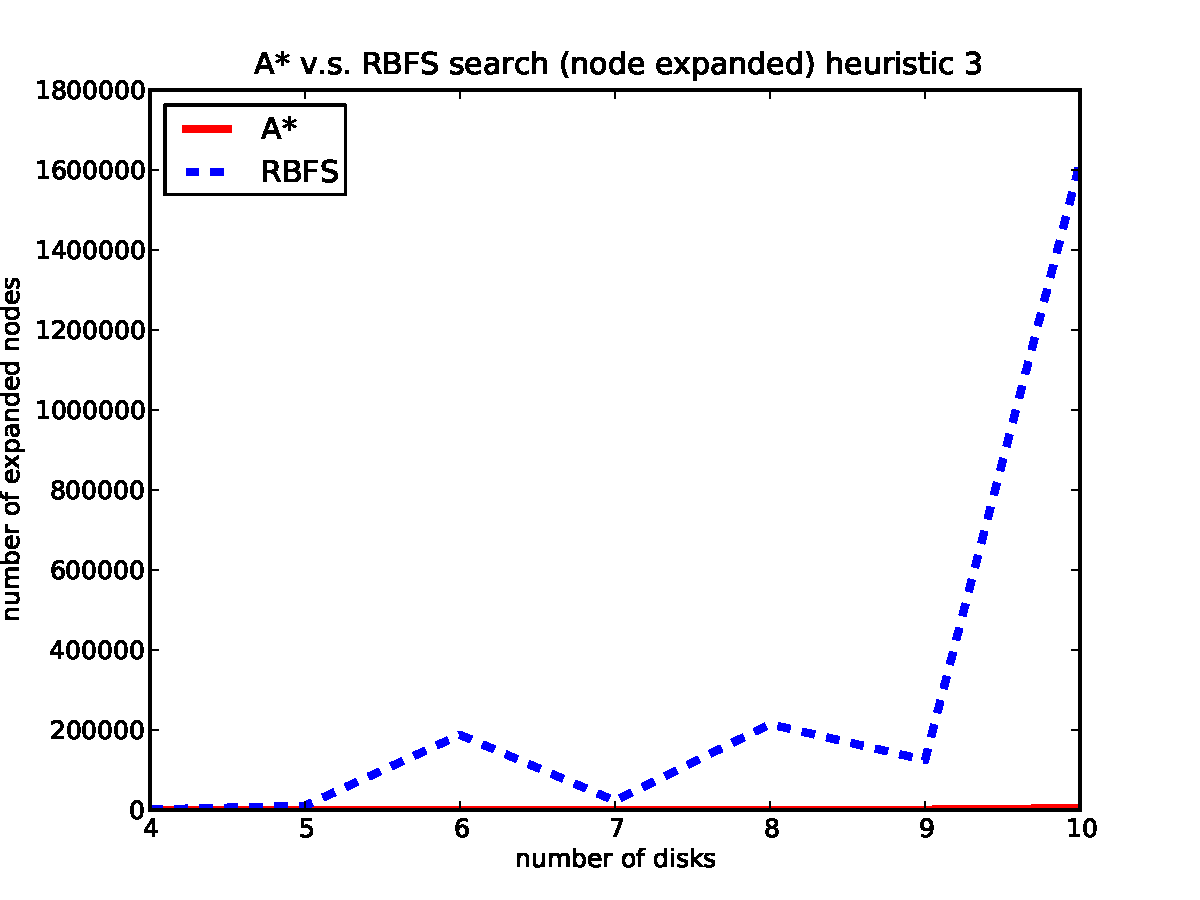
\includegraphics[scale=0.32]{./img/node_Astar_RBFS_H_nad.pdf}}\\
%\subfloat[cpu time against disks for heurisitic 1]{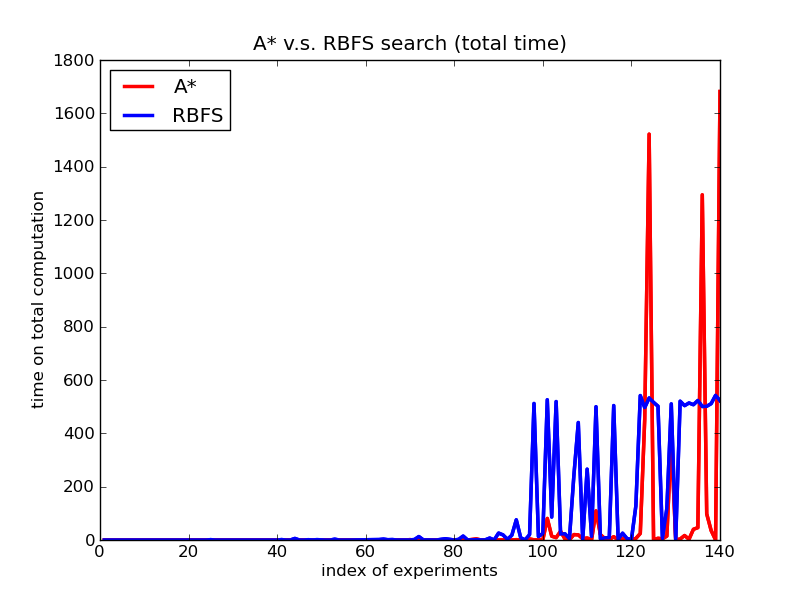
\includegraphics[scale=0.32]{../results/Astar_RBFS_H1_cpu.png}} 
   %& \subfloat[cpu time against disks for heurisitic 2]{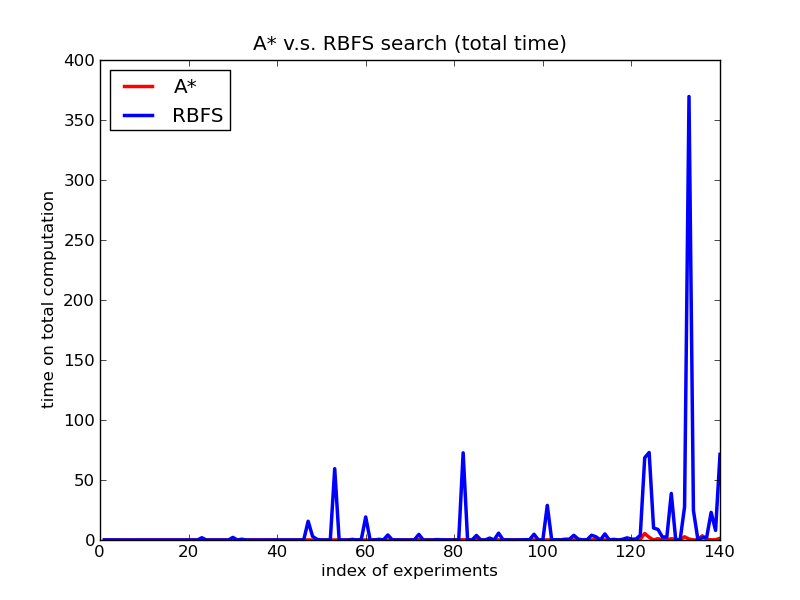
\includegraphics[scale=0.32]{../results/Astar_RBFS_H2_cpu.png}}\\
\end{tabular}
\caption{Performance comparisons between A* and RBFS}
\label{fig:astar-rbfs}
\end{figure}


We tested the three heuristics on all 140 examples for the problem size ranging from $4-10$ with each size having $20$ examples. We couldn't finish the admissible heuristic on the whole data with a ten minute max execution time (which is represented as an NMAX constant, the maximum number of nodes to expand)  per problem. For a large size like $9$ or $10$, a few examples can take more than one hour. For RBFS, the number of expanded nodes grew rapidly and failed the NMAX constraint. We show the results on disk sizes $4-9$ for the admissible heuristic (heuristic 1) and the whole data for non-admissible heuristics (heuristic 2 and 3). 

The first and second experiments are comparisons of the number of expanded nodes and cpu time between different heurisitics, which are shown in figure \ref{fig:nodes} and figure \ref{fig:cputime} respectively. We can see that both nodes and cpu time grow up expenentially. However, a well-designed heuristic function can control the increase in a certain range. It may not necessarily lead to an optimal solution but it is efficient for a real-time problem. 

We also compared A* and RBFS (figure \ref{fig:astar-rbfs}): we found that the trends of number of expanded nodes and cpu time are similar, so we only show the nodes comparison. A* outperforms RBFS in terms of cpu time and searched nodes. From figure \ref{fig:cputime}, we can see RBFS spends $1/3$ of the whole cpu time on heuristic computation while A* takes less than $1$ second. This is because RBFS expands more nodes than A* and every node has to compute a heuristic value.

The average solution lengths are shown in table \ref{tab:solen}. Because some experiments failed in RBFS for reaching the maximum limitation of expanded nodes, the average lengths of the admissible RBFS case are a little bit smaller without these examples, but all values are not far away. It suggests that non-admissible heuristics are also reasonable choices for large scale problems.

\begin{table}[!h]
    \centering
    \scalebox{0.9}{
	    \begin{tabular}{|l|c|c|c|c|c|c|c|}
		\hline
		Disks: & 4 & 5 & 6 & 7 & 8 & 9 & 10\\ \hline
		A*/admissible & 8.8 & 11.6 & 13.95 & 16.5 & 18.6 & n/a & n/a\\ \hline
		%A*/admissible H7 & 8.95 & 11.6 & 13.95 & 16.75 & 19.2 & 22.4 & 24.77\\ \hline
		RBFS/admissible & 8.8 & 11.6 & 13.95 & 16.35 & 17.11 & n/a & n/a\\ \hline
		A*/nonadmissible 1 & 8.85 & 11.85 & 14.6 & 17.5 & 20.2 & 24.1 & 27.6\\ \hline
		RBFS/nonadmissible 1 & 8.85 & 11.85 & 15.25 & 19 & 22.21 & 26.81 & 32.25 \\ \hline
		A*/nonadmissible 2 & 9.25 & 12.95 & 16.5 & 20.05 & 23.8 & 27.4 & 34.05\\ \hline
		RBFS/nonadmissible 2 & 11.25 & 17.85 & 24.35 & 32.75 & 40.35 & 50.7 & 64.55\\ \hline
	    \end{tabular}
    }
    \caption{Average solution length per algorithm, heuristic and disk size. n/a means unable to compute within 10 minutes for all problems. Note that some experiments failed for completing before NMAX nodes; these were not included in the average.}\label{tab:solen}
\end{table}


